In order to assess the influence of interface conditions on the outgassing flux, simulations are performed with chemical potential continuity (Equation \ref{eq: c/s conservation}) or mobile concentration continuity assuming in both cases flux conservation.
For the sake of simplicity and to emphasis on the influence of interface conditions, no trapping was assumed and ideal Dirichlet boundary conditions were set.
Simulations were performed on two test cases: W/Cu and Cu/EUROFER.
The materials properties used for the simulations can be found in Table \ref{tab:materials properties_1}.
In both cases the solute concentration $c_\mathrm{m}$ was set to \SI{1e20}{m^{-3}} at $x=0$ and zero on the other boundary.

% The steady-state temperature field exhibits high temperature gradients between the plasma-facing surface and the cooling surface (see Figure \ref{fig:2D temperature monoblock}).

\begin{figure}
    \centering
    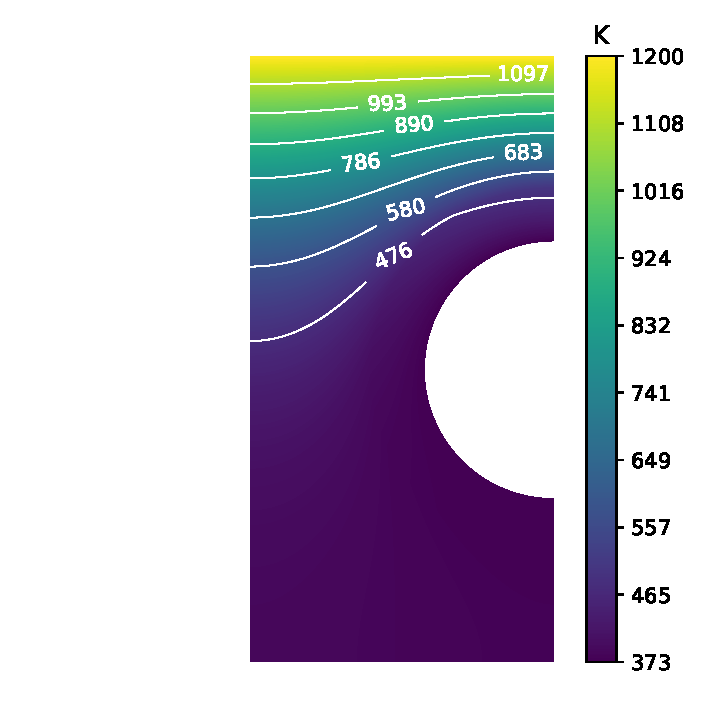
\includegraphics[width=0.8\linewidth]{Figures/Chapter3/monoblocks/interface_condition/iter case/temperature_field_2d.pdf}
    \caption{Steady-state temperature field of an ITER-like monoblock simulated with FESTIM.}
    \label{fig:2D temperature monoblock}
\end{figure}


% TODO replace this figure!!!
\begin{figure}
    \centering
    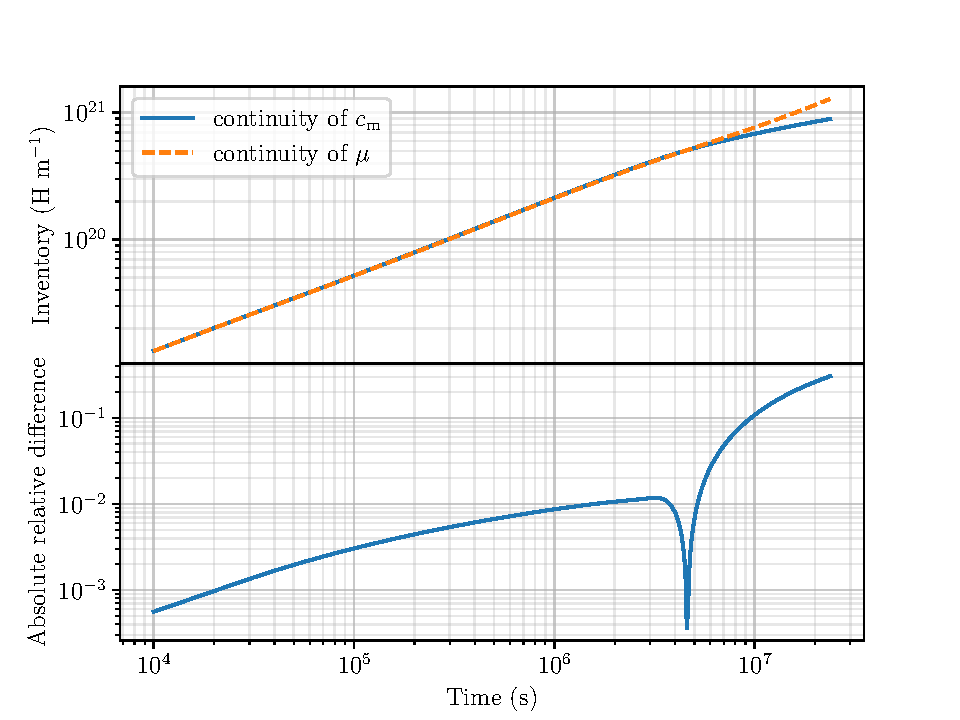
\includegraphics[width=\linewidth]{Figures/Chapter3/monoblocks/interface_condition/iter case/comparison_inventory_2d.pdf}
    \caption{Influence of chemical potential conservation on hydrogen inventory.}
    \label{fig: 2D inventories}
\end{figure}


\begin{figure}
    \centering
    \begin{subfigure}{0.5\linewidth}
        \centering
        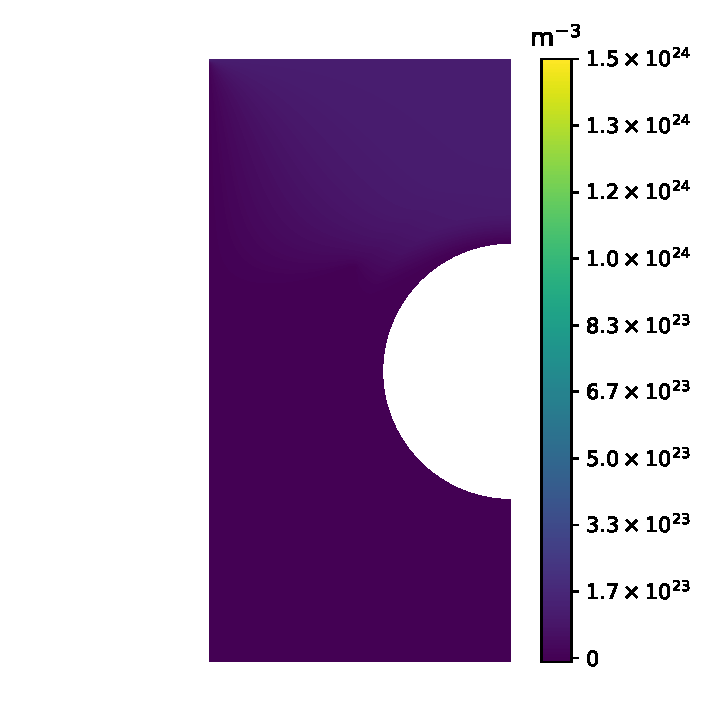
\includegraphics[width=\linewidth]{Figures/Chapter3/monoblocks/interface_condition/iter case/solute_c.pdf}
        \caption{$c_\mathrm{m}$ (continuity of $c_\mathrm{m}$)}
    \end{subfigure}%
    \begin{subfigure}{0.5\linewidth}
        \centering
        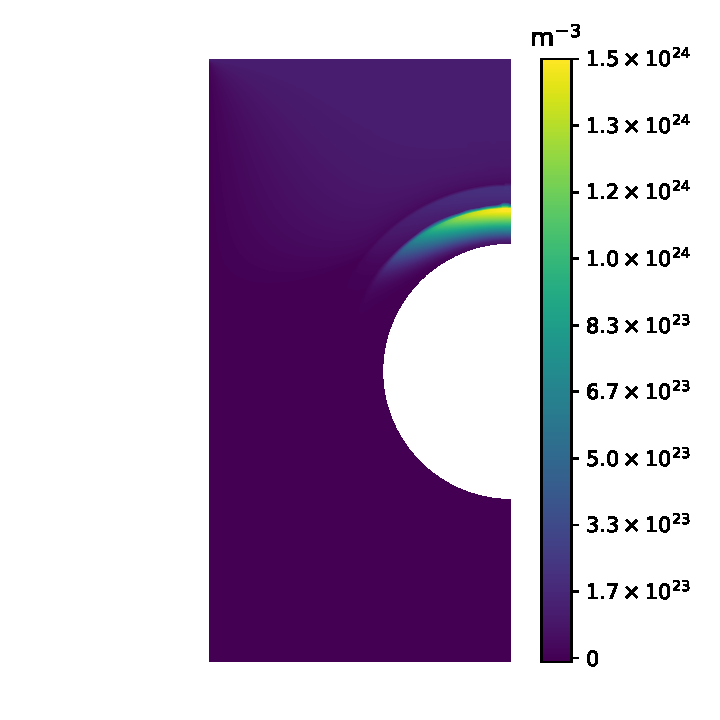
\includegraphics[width=\linewidth]{Figures/Chapter3/monoblocks/interface_condition/iter case/solute_mu.pdf}
        \caption{$c_\mathrm{m}$ (continuity of $\mu$)}
    \end{subfigure}
    \begin{subfigure}{0.5\linewidth}
        \centering
        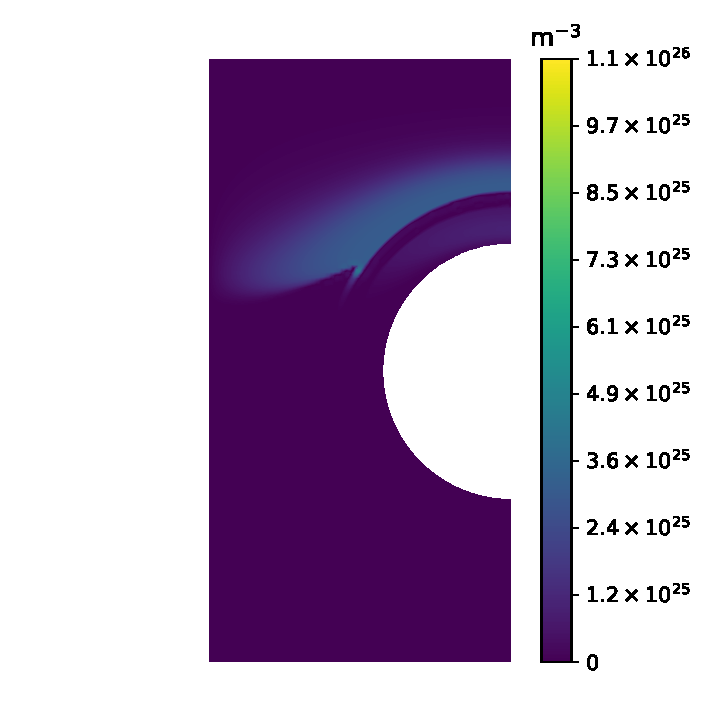
\includegraphics[width=\linewidth]{Figures/Chapter3/monoblocks/interface_condition/iter case/retention_c.pdf}
        \caption{Retention (continuity of $c_\mathrm{m}$)}
    \end{subfigure}%
    \begin{subfigure}{0.5\linewidth}
        \centering
        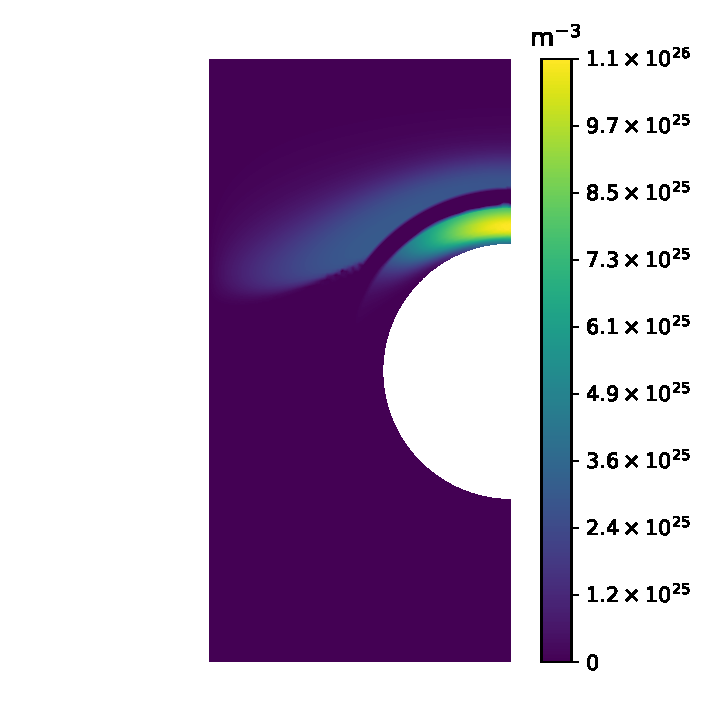
\includegraphics[width=\linewidth]{Figures/Chapter3/monoblocks/interface_condition/iter case/retention_mu.pdf}
        \caption{Retention (continuity of $\mu$)}
    \end{subfigure}
    \caption{2D concentration fields at $t=\SI{2.4e7}{s}$}
    \label{fig: concentrations fields 2d}
\end{figure}
Two cases were examined, one with mobile concentration $c_\mathrm{m}$ continuity at interfaces and the other with continuity of chemical potential (\textit{ie.} continuity of $c_\mathrm{m}/S$).

Up to \SI{5e6}{s}, there was no difference in the total hydrogen inventory between the two cases (see Figure \ref{fig: 2D inventories}).
It is only after this implantation that the inventory of the two cases started to diverge.
At $t=\SI{2.4e7}{s}$, the inventory of the continuity of chemical potential case was higher than with continuity of $c_\mathrm{m}$.
This is explained by the high solubility ratio between Cu and CuCrZr leading to a higher concentration of mobile particles in CuCrZr and therefore a higher trapping rate.
However, even then, the trap density in Cu being low compared to other materials, the global inventory is not affected much.
For these two reasons, the inventories are unaffected before \SI{5e6}{s}.

Similarily, before reaching the W/Cu interface, the $c_\mathrm{m}$ and retention profiles are identical regardless of the interface condition (see Figure \ref{fig: concentrations fields 2d}).
Once the W/Cu interface is reached, the $c_\mathrm{m}$ profiles are affected by the interface condition.
The interface condition had no influence whatsoever on the mobile particle concentration $c_\mathrm{m}$ in the W.
However, $c_\mathrm{m}$ was higher in Cu and CuCrZr in the case with chemical potential conservation (up to \SI{1.5e24}{m^{-3}} in CuCrZr at $t=\SI{2.4e7}{s}$).
This increase of $c_\mathrm{m}$ leads to an increase of the trap occupancy and therefore an increase of the local retention.

The retro-desorbed flux (from the monoblock to the plasma) does not depend on the interface conditions since interfaces are far from the exposed surface.
Moreover, outgassing flux through the cooling pipe greatly depends on the boundary condition imposed at the cooling surface.
Therefore, in order to assess the impact of interface conditions on the outgassing flux through the cooling pipe, uncertainties must first be lift regarding the recombination process occurring on surfaces in contact with water.

% \subsection{Summary}
% should we keep this
% The influence of interface conditions between materials has been studied with FESTIM.
% A novel approach has been implemented in FESTIM in order to ensure equilibrium at the interfaces.
% The implementation has been verified using the Method of Exact Solutions and the Method of Manufactured Solutions.
% % A comparison test has been performed with TMAP7 and Abaqus and the three codes show very good agreement.

% H transport through Cu/EUROFER and W/Cu composite slabs has been studied.
% It is shown that the interface condition can have an impact on the outgassing flux.
% This modelling work will help design future permeation barriers in DEMO.
% A method for identifying material properties with either an analytical solution or with the FESTIM code is also described.

% The influence of interface conditions is also studied on the ITER monoblock test case in both 1D and 2D.
% It is shown that this has very low influence up to \SI{5e6}{s} and that discrepancies only start to appear after a very long exposure time.
% This is because interfaces are far from the exposed surface and hydrogen atoms only reach these interface after a long exposure time.
% The continuity of mobile concentration can therefore be employed safely for monoblocks H transport simulations in order to assess monoblocks inventory.
% This is especially true when desorption is assumed on the edges of the monoblock where less H particles will reach the interfaces.
% In other words, the effect of the interfaces conditions is negligible compared to the edge effects (this will be shown in more details in Section \ref{3D edge effects}).
